\chapter{VARIATIONAL AUTOENCODERS}
\begin{onehalfspacing}
    Autoencoders are unsupervised neural networks that can learn efficient 
    data encodings. Autoencoders learn the representation for the data, 
    typically for dimensionality reduction. Initially, an autoencoder 
    compresses the input data into a latent vector. The latent vector can be 
    used to regenerate the input data later. Traditionally, autoencoders were 
    used for dimensionality reduction and feature learning. In the recent times, 
    autoencoders are being used to learn generative models of data.
    
    \begin{figure}[h]
        \centering
        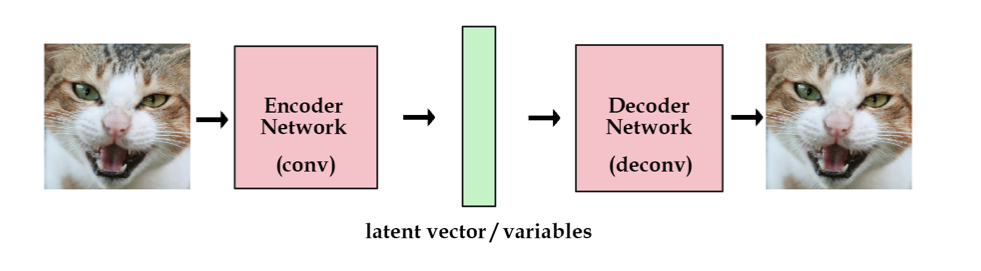
\includegraphics[width=0.8\linewidth]{images/autoencoders.png}
        \caption{Autoencoders \cite{autoencoders_image}}
        \label{fig:autoencoders}
    \end{figure} 

    The autoencoder \ref{fig:autoencoders} has two component neural networks, 
    an encoder and a decoder. The encoder neural network can be represented by 
    $h = f(x)$.  The decoder, $r = g(h)$ produces a reconstruction.
    An autoencoder will be not useful if it simply replicates the input given 
    to it. Thus, the autoencoder is not allowed to copy the input directly 
    instead it learns useful parameters from the input  \cite{dlbook}. 

\end{onehalfspacing}